\documentclass{beamer}

\mode<presentation>

\usepackage{dirtree}
\usepackage{ifthen}
\usepackage[utf8]{inputenc}
\usepackage{listings}
\usepackage{minted}
\usepackage{xcolor}
\usepackage{xifthen}

\setbeamertemplate{footline}[frame number]
\usetheme{Singapore}
\usecolortheme{seagull}
\newenvironment{Frame}{\begin{frame}[containsverbatim]{\subsecname}}{\end{frame}}
\newenvironment{FrameTP}{\begin{frame}[containsverbatim]{\secname}}{\end{frame}}

\lstdefinestyle{lst_base_style}{
    language=C,
    numbers=left,
    basicstyle=\ttfamily,
    keywordstyle=\color{blue}\ttfamily,
    identifierstyle=\color{brown}\ttfamily,
    stringstyle=\color{teal}\ttfamily,
    commentstyle=\color{gray}\ttfamily
}
\lstset{style=lst_base_style, texcl=true}
\newcommand{\PrintSnippet}[5]{
    \ifthenelse{\isempty{#5}}
    {
        \lstinputlisting[title=#2, language=#1]{#3}
    }
    {
        \lstinputlisting[title=#2,
            firstline=#4, lastline=#5, firstnumber=#4
        ]{#3}
    }
}
\newcommand{\ProjectView}[2]{
    \begin{columns}[T]
        \column{\dimexpr \paperwidth-0.8\textwidth}
        #1
        \column{0.8\textwidth}   
        \tiny
        #2
    \end{columns}
}
\newcommand{\SectionFrame}[0]{
    \begin{frame}
        \centering
        \Large
        \textbf{\secname}
    \end{frame}
}

\title{Introduction au moteur de production CMake}

\author{
   
\includegraphics[height=3cm]{CMake_Logo.png}
}

\begin{document}

\begin{frame}
    \maketitle
\end{frame}

\begin{frame}
    \tiny
    \tableofcontents
\end{frame}

\section{\textit{GNU toolchain}}

\SectionFrame

\subsection{Les étapes de compilation}

\begin{Frame}
    \PrintSnippet{C}{Fichier source (\texttt{main.c})}{main.c}{}{}
\end{Frame}

\begin{Frame}
    \PrintSnippet{C}{Après l'étape de \textit{preprocessing} (\texttt{main.i})}{main.i}{}{}
\end{Frame}

\begin{Frame}
    \small
    \PrintSnippet{C}{Après compilation (\texttt{main.S})}{main.S}{5}{18}
\end{Frame}

\begin{Frame}
    \PrintSnippet{C}{Après assemblage  (\texttt{main.o})}{main_dump.txt}{}{}
\end{Frame}

\begin{Frame}
    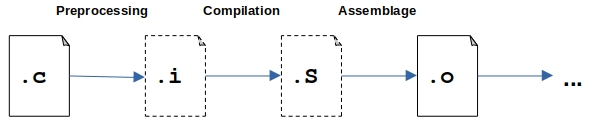
\includegraphics[width=\textwidth]{compilation_to_obj.jpg}
\end{Frame}

\subsection{Fonctionnement des entêtes}

\begin{Frame}
    \setlength{\DTbaselineskip}{1em}
    \ProjectView{
        \dirtree{%
            .1 project/.
                .2 main.c.
                .2 aux.c.
        }
    }{
        \PrintSnippet{C}{\texttt{main.c}}{main_for_aux.c}{}{}
        \PrintSnippet{C}{\texttt{aux.c}}{aux.c}{}{}
    }
\end{Frame}

\begin{Frame}
\begin{minted}[breaklines]{bash}
$ gcc aux.c main_for_aux.c
main_for_aux.c: In function ‘main’:
main_for_aux.c:4:29: warning: implicit declaration of function ‘my_function’ [-Wimplicit-function-declaration]
    4 |   printf("My value = %d\n", my_function());
      |                             ^~~~~~~~~~~
$ ./a.out
hello
My value = 6
\end{minted}
\end{Frame}

\begin{Frame}
    \setlength{\DTbaselineskip}{1em}
    \begin{columns}[T]
        \column{\dimexpr \paperwidth-0.8\textwidth}   
        \dirtree{%
            .1 project/.
                .2 main.c.
                .2 aux.c.
                .2 aux.h.
        }
        
        \column{0.8\textwidth}
        \tiny
        \PrintSnippet{C}{\texttt{main.c}}{main_for_aux_fixed.c}{}{}
        \vspace{-2em}
        \PrintSnippet{C}{\texttt{aux.c}}{aux_fixed.c}{}{}
        \vspace{-2em}
        \PrintSnippet{C}{\texttt{aux.h}}{aux.h}{}{}
    \end{columns}
\end{Frame}

\begin{Frame}
\begin{minted}[breaklines]{bash}
$ gcc aux.c main_for_aux.c
main_for_aux.c: In function ‘main’:
main_for_aux.c:6:29: error: invalid use of void expression
    6 |   printf("My value = %d\n", my_function());
      |
\end{minted}
\end{Frame}

\begin{Frame}
    \begin{columns}
        \column{0.5\textwidth}
        \centering
        \textbf{Avec entêtes}
        \begin{itemize}
            \item \textbf{Traditionnellement}, les entêtes contiennent les \textbf{déclarations} des fonctions
            \item Souvent appairées avec des fichiers sources, qui contiennent les \textbf{définitions}
            \item Besoin de synchroniser l'entête avec son fichier source
            \item Système utilisé par les langages relativement vieux (C, C++, ...) 
        \end{itemize}

        \column{0.5\textwidth}
        \centering
        \textbf{Sans entêtes}
        \begin{itemize}
            \item Les fichiers sources contiennent les \textbf{définitions} des fonctions et peuvent être "inclus" directement.
            \item Les fichiers sources se suffisent à eux-mêmes
            \item Système utilisé par les langages récents (Python, Java, Rust, C++, ...)
        \end{itemize}
    \end{columns}
\end{Frame}

\subsection{Linkage}

\begin{Frame}
    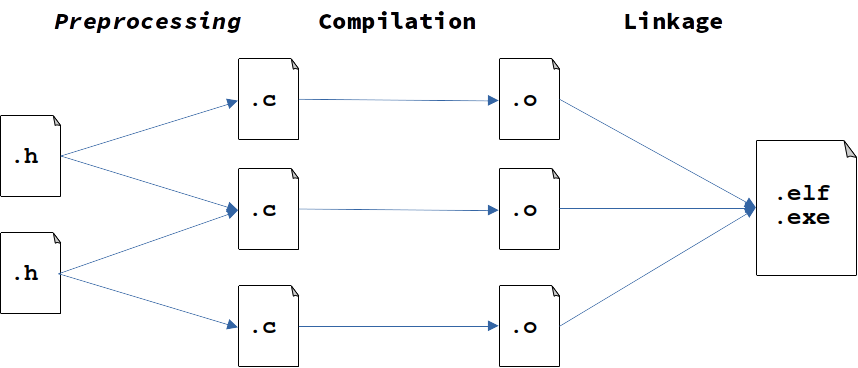
\includegraphics[width=\textwidth]{compilation_steps.png}
\end{Frame}

\section{GNU Make}

\SectionFrame

\subsection{Principe}

\begin{Frame}
    \centering
    Structure d'une règle
    \begin{lstlisting}
        cible: dependances...
            recette...
    \end{lstlisting}
    Exemple
    \begin{lstlisting}
        application: main.o aux.o
            gcc main.o aux.o
    \end{lstlisting}
\end{Frame}

\begin{Frame}
    \setlength{\DTbaselineskip}{1em}
    \ProjectView{
        \dirtree{%
            .1 project/.
                .2 main.c.
                .2 aux.c.
                .2 aux.h.
                .2 Makefile.
        }
    }{
        \PrintSnippet{make}{Makefile}{Makefile}{1}{2}
        (Règle pour générer \texttt{main.o} ?) \\
        (Règle pour générer \texttt{aux.o} ?)
    }
\end{Frame}

\begin{Frame}
    \setlength{\DTbaselineskip}{1em}
    \ProjectView{
        \dirtree{%
            .1 project/.
                .2 main.c.
                .2 aux.c.
                .2 aux.h.
                .2 Makefile.
        }
    }{
        \PrintSnippet{make}{Makefile}{Makefile}{1}{5}
        (Règle pour générer \texttt{aux.o} ?)
    }
\end{Frame}

\begin{Frame}
    \setlength{\DTbaselineskip}{1em}
    \ProjectView{
        \dirtree{%
            .1 project/.
                .2 main.c.
                .2 aux.c.
                .2 aux.h.
                .2 Makefile.
        }
    }{
        \PrintSnippet{make}{Makefile}{Makefile}{1}{8}
    }
\end{Frame}

\subsection{Relation avec CMake}

\begin{Frame}
    \begin{columns}
        \column{0.5\textwidth}
        \centering
        \textbf{GNU Make}
        \begin{itemize}
            \item \textit{Build system}
            \item Permet de produire des \textbf{binaires} (exécutables, bibliothèques statiques et dynamiques...)
        \end{itemize}

        \column{0.5\textwidth}
        \centering
        \textbf{CMake}
        \begin{itemize}
            \item Générateur de \textit{build systems}
            \item Permet de générer des \textbf{Makefiles}
        \end{itemize}
    \end{columns}

    \vspace{2em}

    \begin{center}   
        \textbf{CMake s'utilise donc avec Makefile (ou un autre \textit{build system})}
    \end{center}
\end{Frame}

\section{CMake}

\SectionFrame

\subsection{Le \textit{source tree} et le \textit{binary tree}}

\begin{Frame}
    \setlength{\DTbaselineskip}{1em}
    \begin{columns}
        \column{0.5\textwidth}
        \begin{center}   
            \textit{Source tree}
        \end{center}
        \dirtree{%
            .1 project/.
                .2 CMakeLists.txt.
                .2 main.c.
                .2 src/.
                    .3 CMakeLists.txt.
                    .3 aux\_a.c.
                    .3 aux\_b.c.
                .2 include/.
                    .3 CMakeLists.txt.
                    .3 aux\_a.h.
                    .3 aux\_b.h.
        }
        
        \column{0.5\textwidth}
        \begin{center}   
            \textit{\textbf{Binary tree ?}}
        \end{center}
    \end{columns}
\end{Frame}

\begin{Frame}
    \setlength{\DTbaselineskip}{1em}
    \begin{columns}
        \column{0.5\textwidth}
        \begin{center}   
            \textit{Source tree}
        \end{center}
        \dirtree{%
            .1 project/.
                .2 CMakeLists.txt.
                .2 main.c.
                .2 src/.
                    .3 CMakeLists.txt.
                    .3 aux\_a.c.
                    .3 aux\_b.c.
                .2 include/.
                    .3 CMakeLists.txt.
                    .3 aux\_a.h.
                    .3 aux\_b.h.
        }
        
        \column{0.5\textwidth}
        \begin{center}
            \textit{Binary tree}
        \end{center}
        \dirtree{%
            .1 build/.
                .2 Makefile.
                .2 MyExecutable.
                .2 src/.
                    .3 Makefile.
                    .3 libMyLibrary.a.
                .2 include/.
                    .3 Makefile.
        }

        Note: en réalité, le \textit{binary tree} comporte plus de fichiers, mais par souci de clarté, seuls les fichiers principaux ont été gardé.
    \end{columns}
\end{Frame}

\begin{Frame}
    \setlength{\DTbaselineskip}{0.6em}
    \footnotesize
    \dirtree{%
        .1 project/.
            .2 CMakeLists.txt.
            .2 main.c.
            .2 build/ \ldots{}
                \begin{minipage}[t]{7cm}
                    En général, le \textit{binary tree} se trouve dans un dossier nommé \texttt{build/} situé à la racine du projet
                \end{minipage}.
                .3 Makefile.
                .3 MyExecutable.
                .3 src/.
                    .4 Makefile.
                    .4 libMyLibrary.a \ldots{}
                        \begin{minipage}[t]{4cm}
                            \textbf{Bibliothèque statique}
                        \end{minipage}.
                .3 include/.
                    .4 Makefile.
            .2 src/.
                .3 CMakeLists.txt.
                .3 aux\_a.c.
                .3 aux\_b.c.
            .2 include/.
                .3 CMakeLists.txt.
                .3 aux\_a.h.
                .3 aux\_b.h.
    }   
\end{Frame}

\subsection{L'étape de configuration et de génération}

\begin{Frame}
    \setlength{\DTbaselineskip}{1em}
    Commande:
    \begin{minted}{bash}
$ cmake -B build
    \end{minted}

    \textbf{Résultat ?}
    \begin{columns}
        \column{0.5\textwidth}
        \begin{center}   
            \textit{Source tree}
        \end{center}
        \dirtree{%
            .1 project/.
                .2 CMakeLists.txt.
                .2 main.c.
                .2 src/.
                    .3 CMakeLists.txt.
                    .3 aux\_a.c.
                    .3 aux\_b.c.
                .2 include/.
                    .3 CMakeLists.txt.
                    .3 aux\_a.h.
                    .3 aux\_b.h.
        }
        
        \column{0.5\textwidth}
        \begin{center}   
            \textit{Binary tree}
        \end{center}
        \dirtree{%
            .1 build/.
                .2 \textbf{????????}.
                .2 src/.
                    .3 \textbf{????????}.
                .2 include/.
                    .3 \textbf{????????}.
        }
    \end{columns}
\end{Frame}

\begin{Frame}
    \setlength{\DTbaselineskip}{1em}
    Commande:
    \begin{minted}{bash}
$ cmake -B build
    \end{minted}

    Résultat:
    \begin{columns}
        \column{0.5\textwidth}
        \begin{center}   
            \textit{Source tree}
        \end{center}
        \dirtree{%
            .1 project/.
                .2 CMakeLists.txt.
                .2 main.c.
                .2 src/.
                    .3 CMakeLists.txt.
                    .3 aux\_a.c.
                    .3 aux\_b.c.
                .2 include/.
                    .3 CMakeLists.txt.
                    .3 aux\_a.h.
                    .3 aux\_b.h.
        }
        
        \column{0.5\textwidth}
        \begin{center}   
            \textit{Binary tree}
        \end{center}
        \dirtree{%
            .1 build/.
                .2 Makefile.
                .2 src/.
                    .3 Makefile.
                .2 include/.
                    .3 Makefile.
        }
    \end{columns}
\end{Frame}

\subsection{L'étape de construction du projet}

\begin{Frame}
    \setlength{\DTbaselineskip}{1em}
    Commande:
    \begin{minted}{bash}
$ cmake --build build OU $ make -C build
    \end{minted}

    \textbf{Résultat ?}
    \begin{columns}
        \column{0.5\textwidth}
        \begin{center}   
            \textit{Source tree}
        \end{center}
        \dirtree{%
            .1 project/.
                .2 CMakeLists.txt.
                .2 main.c.
                .2 src/.
                    .3 CMakeLists.txt.
                    .3 aux\_a.c.
                    .3 aux\_b.c.
                .2 include/.
                    .3 CMakeLists.txt.
                    .3 aux\_a.h.
                    .3 aux\_b.h.
        }
        
        \column{0.5\textwidth}
        \begin{center}   
            \textit{Binary tree}
        \end{center}
        \dirtree{%
            .1 build/.
                .2 Makefile.
                .2 \textbf{????????????}.
                .2 src/.
                    .3 Makefile.
                    .3 \textbf{??????????????}.
                .2 include/.
                    .3 Makefile.
        }
    \end{columns}
\end{Frame}

\begin{Frame}
    \setlength{\DTbaselineskip}{1em}
    Commande:
    \begin{minted}{bash}
$ cmake --build build OU $ make -C build
    \end{minted}

    Résultat:
    \begin{columns}
        \column{0.5\textwidth}
        \begin{center}   
            \textit{Source tree}
        \end{center}
        \dirtree{%
            .1 project/.
                .2 CMakeLists.txt.
                .2 main.c.
                .2 src/.
                    .3 CMakeLists.txt.
                    .3 aux\_a.c.
                    .3 aux\_b.c.
                .2 include/.
                    .3 CMakeLists.txt.
                    .3 aux\_a.h.
                    .3 aux\_b.h.
        }
        
        \column{0.5\textwidth}
        \begin{center}   
            \textit{Binary tree}
        \end{center}
        \dirtree{%
            .1 build/.
                .2 Makefile.
                .2 MyExecutable.
                .2 src/.
                    .3 Makefile.
                    .3 libMyLibrary.a.
                .2 include/.
                    .3 Makefile.
        }
    \end{columns}
\end{Frame}

\section{Commandes pour le TP}

\SectionFrame

\subsection{\texttt{add\_executable}}

\begin{Frame}
    \setlength{\DTbaselineskip}{1em}
    Contenu de \texttt{CMakeLists.txt}:
    \begin{minted}{cmake}
add_executable(MyExecutable main.c aux.c)
    \end{minted}

    Résultat:
    \begin{columns}
        \column{0.5\textwidth}
        \begin{center}   
            \textit{Source tree}
        \end{center}
        \dirtree{%
            .1 project/.
                .2 CMakeLists.txt.
                .2 main.c.
                .2 aux.c.
        }
        
        \column{0.5\textwidth}
        \begin{center}   
            \textit{Binary tree}
        \end{center}
        \dirtree{%
            .1 build/.
                .2 Makefile.
                .2 MyExecutable.
        }
    \end{columns}
\end{Frame}

\subsection{\texttt{add\_library}}

\begin{Frame}
    \setlength{\DTbaselineskip}{1em}
    Contenu de \texttt{CMakeLists.txt}:
    \begin{minted}{cmake}
add_library(MyLibrary aux_a.c aux_b.c aux_c.c)
    \end{minted}

    Résultat:
    \begin{columns}
        \column{0.5\textwidth}
        \begin{center}   
            \textit{Source tree}
        \end{center}
        \dirtree{%
            .1 project/.
                .2 CMakeLists.txt.
                .2 aux\_a.c.
                .2 aux\_b.c.
                .2 aux\_c.c.
        }
        
        \column{0.5\textwidth}
        \begin{center}   
            \textit{Binary tree}
        \end{center}
        \dirtree{%
            .1 build/.
                .2 Makefile.
                .2 libMyLibrary.a.
        }
    \end{columns}
\end{Frame}

\subsection{\texttt{target\_include\_directories}}

\begin{Frame}
    \setlength{\DTbaselineskip}{0.8em}
    Contenu de \texttt{include/CMakeLists.txt}:
    
    \footnotesize
    \begin{minted}{cmake}
target_include_directories(MyLibrary PUBLIC ${CMAKE_CURRENT_SOURCE_DIR})
    \end{minted}
    
    (Hypothèse : \texttt{src/CMakeLists.txt} définit la bibliothèque \verb|MyLibrary|)
    
    \normalsize
    Résultat:
    \begin{columns}
        \column{0.5\textwidth}
        \begin{center}   
            \textit{Source tree}
        \end{center}
        \footnotesize
        \dirtree{%
            .1 project/.
                .2 CMakeLists.txt.
                .2 src/.
                    .3 CMakeLists.txt.
                    .3 aux\_a.c.
                    .3 aux\_b.c.
                    .3 aux\_c.c.
                .2 include/.
                    .3 CMakeLists.txt.
                    .3 aux\_a.h.
                    .3 aux\_b.h.
                    .3 aux\_c.h.
        }

        \column{0.5\textwidth}
        Aucun résultat visible dans le \textit{build tree}... Cela permet juste d'indiquer au compilateur où se trouvent les entêtes associées à la bibliothèque \verb|MyLibrary|.
        \verb|${CMAKE_CURRENT_SOURCE_DIR}| est égale au chemin du dossier qui contient le \verb|CMakeLists.txt| en cours d'évaluation.
    \end{columns}
\end{Frame}

\subsection{\texttt{target\_link\_libraries}}

\begin{Frame}
    \setlength{\DTbaselineskip}{0.3em}
    Contenu de \texttt{CMakeLists.txt}:
    
    \footnotesize
    \begin{minted}{cmake}
add_executable(MyExecutable main.c)
target_link_libraries(MyExecutable PUBLIC MyLibrary)
    \end{minted}
    
    (Hypothèses : \texttt{src/CMakeLists.txt} définit la bibliothèque \verb|MyLibrary| et \texttt{include/CMakeLists.txt} déclare \texttt{include/} comme chemin d'inclusion pour \texttt{MyLibrary})

    \normalsize
    Résultat:
    \begin{columns}
        \column{0.5\textwidth}
        \footnotesize
        \begin{center}   
            \textit{Source tree}
        \end{center}
        \dirtree{%
            .1 project/.
                .2 CMakeLists.txt.
                .2 main.c.
                .2 src/.
                    .3 CMakeLists.txt.
                    .3 aux\_a.c.
                    .3 aux\_b.c.
                    .3 aux\_c.c.
                .2 include/.
                    .3 CMakeLists.txt.
                    .3 aux\_a.h.
                    .3 aux\_b.h.
                    .3 aux\_c.h.
        }

        \column{0.5\textwidth}
        Aucun résultat visible... Cette commande permet d'indiquer au compilateur de linker notre exécutable avec notre bibliothèque, mais aussi d'ajouter les chemins d'inclusions de \texttt{MyLibrary} à \texttt{MyExecutable}.
    \end{columns}
\end{Frame}

\subsection{\texttt{add\_subdirectory}}

\begin{Frame}
    \setlength{\DTbaselineskip}{0.8em}
    Contenu de \texttt{CMakeLists.txt}:
    
    \begin{minted}{cmake}
add_subdirectory(src)
add_subdirectory(include)
    \end{minted}

    Résultat:
    \begin{columns}
        \column{0.5\textwidth}
        \begin{center}   
            \textit{Source tree}
        \end{center}
        \footnotesize
        \dirtree{%
            .1 project/.
                .2 CMakeLists.txt.
                .2 src/.
                    .3 CMakeLists.txt.
                .2 include/.
                    .3 CMakeLists.txt.
        }

        \column{0.5\textwidth}
        \begin{center}   
            \textit{Binary tree}
        \end{center}
        \dirtree{%
            .1 project/.
                .2 Makefile.
                .2 src/.
                    .3 Makefile.
                .2 include/.
                    .3 Makefile.
        }
    \end{columns}
\end{Frame}

\section{TP: Projet CMake basique}

\SectionFrame

\begin{FrameTP}
    Clonez le dépot :
    \begin{minted}{bash}
git clone https://github.com/Club-INTech/Formation-CMake
    \end{minted}
    et \textbf{écrivez un ou plusieurs fichier(s) \texttt{CMakeLists.txt} afin de pouvoir construire le projet}.
    
    Il y a plusieurs solutions possibles, mais le but de l'exercice est d'y parvenir \textbf{sans modifier les fichiers sources}.
    
    Pour vérifier votre solution, lancez l'exécutable obtenu.
\end{FrameTP}

\section{FetchContent}

\subsection{Déclarer une dépendance externe avec \texttt{FetchContent\_Declare}}

\begin{Frame}
    \setlength{\DTbaselineskip}{1em}
    Contenu de \texttt{CMakeLists.txt}:
    
    \begin{minted}{cmake}
include(FetchContent)
FetchContent_Declare(
    ExternalDependency
    GIT_REPOSITORY https://github.com/boostorg/boost)
    \end{minted}

    Résultat:
    \begin{columns}
        \column{0.5\textwidth}
        \begin{center}   
            \textit{Source tree}
        \end{center}
        \dirtree{%
            .1 project/.
                .2 CMakeLists.txt.
        }

        \column{0.5\textwidth}
        \footnotesize
        Aucun résultat visible... Cette ligne permet de déclarer et de décrire une dépendance via FetchContent (ici, un projet CMake hébergé sur GitHub). Cependant, \textbf{la dépendance n'est pas téléchargée} tant qu'elle n'est pas requise.
    \end{columns}
\end{Frame}

\subsection{Solliciter une dépendance externe pour l'utiliser avec \texttt{FetchContent\_MakeAvailable}}

\begin{Frame}
    \setlength{\DTbaselineskip}{0.5em}
    Contenu de \texttt{CMakeLists.txt}:
    
    \begin{minted}{cmake}
include(FetchContent)
FetchContent_Declare(
    ExtLib
    GIT_REPOSITORY https://github.com/boostorg/boost)
FetchContent_MakeAvailable(ExtLib)
    \end{minted}

    Résultat:
    \begin{columns}
        \column{0.5\textwidth}
        \begin{center}   
            \textit{Source tree}
        \end{center}
        \dirtree{%
            .1 project/.
                .2 CMakeLists.txt.
        }

        \column{0.5\textwidth}
        \begin{center}   
            \textit{Binary tree}
        \end{center}
        \footnotesize
        \dirtree{%
            .1 build/.
                .2 \_deps/.
                    .3 extlib-build/.
                    .3 extlib-src/.
                    .3 extlib-subbuild/.
        }
    \end{columns}
\end{Frame}

\subsection{Exercice rapide}

\begin{Frame}
    Si vous n'avez pas trouvé de solution à l'exercice précédent, vous pouvez en télécharger une depuis le dépôt.
\begin{minted}{bash}
git reset HEAD --hard # Efface toutes vos modifications
git checkout ex2      # Avance jusqu'à l'exercice 2
\end{minted}

   Ensuite, modifier les \texttt{CMakeLists.txt} afin de pouvoir indiquer à FetchContent de télécharger la branche \texttt{external} du dépôt, et linker la bibliothèque ainsi téléchargée à votre exécutable.
   \begin{minted}{cmake}
FetchContent_Declare(
    <nom pour désigner la dépendance>
    GIT_REPOSITORY <lien vers le dépôt git>
    GIT_TAG <nom de la branche à télécharger>
)
   \end{minted}
\end{Frame}

\section{Conclusion}

\subsection{Et après ?}

\begin{Frame}
    \begin{itemize}
        \item \verb|add_custom_target| et \verb|add_custom_command| pour créer vos propres cibles et règles
        \item \verb|set| et \verb|list| pour manipuler les variables
        \item Les fonctions, les structures \verb|if| et \verb|for|
        \item \verb|include|, \verb|CMAKE_MODULE_PATH| pour créer et utiliser des modules CMake
    \end{itemize}
\end{Frame}

\end{document}
